% -*- LaTeX -*-
% -*- coding: utf-8 -*-
%
% ~~~~~~~~~~~~~~~~~~~~~~~~~~~~~~~~~~~~~~~~~~~~~~~~~~~~~~~~~~~~~~~~~~~~~~~~~~~~~~
%
%                             michael a.g. aïvázis
%                      california institute of technology
%                      (c) 1998-2010  all rights reserved
%
% ~~~~~~~~~~~~~~~~~~~~~~~~~~~~~~~~~~~~~~~~~~~~~~~~~~~~~~~~~~~~~~~~~~~~~~~~~~~~~~
%

\lecture{}{20100120}

% --------------------------------------
% threads and shared memory parallelism 
\begin{frame}[fragile]
%
  \frametitle{Threads and shared memory parallelism}
%
  \begin{itemize}
%
  \item recall the shared memory architecture
%
    \begin{figure}
      \centering
      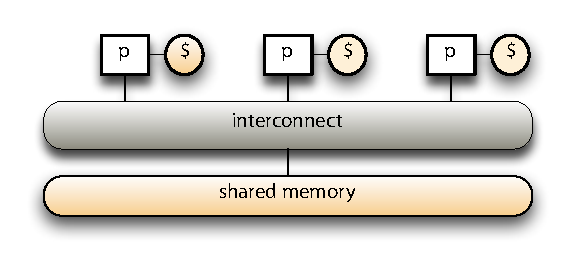
\includegraphics[scale=0.5]{figures/shared-memory.pdf}
    \end{figure}
    \vspace{-1.0em}
%
    \begin{itemize}
    \item processors are connected to a memory pool with a global address space
    \item processors have their own cache but no private memory
    \end{itemize}
%
  \item most modern operating provide threads
%
    \begin{itemize}
    \item lightweight processes that can be scheduled independently, but share many OS
      resources
      \begin{itemize}
      \item CPU
      \item memory
      \item but also file descriptors, process environment, etc.
      \end{itemize}
    \end{itemize}
%
    \begin{figure}
      \centering
      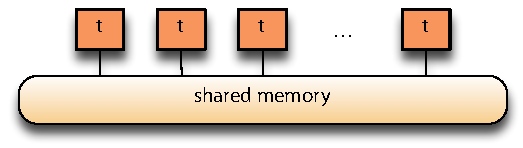
\includegraphics[scale=0.5]{figures/threads-memory.pdf}
    \end{figure}
%
  \end{itemize}
%
\end{frame}

% end of file 
